%% Position, not importance: what a likelihood threshold actually defers on
%% arXiv preprint style. Build: pdflatex paper.tex (twice).
\documentclass[10pt]{article}
\usepackage[a4paper,margin=0.95in,headheight=14pt]{geometry}
\usepackage[T1]{fontenc}
\usepackage[utf8]{inputenc}
\usepackage{times}
\usepackage{microtype}
\usepackage{amsmath,amssymb}
\usepackage{graphicx}
\usepackage{booktabs}
\usepackage{xcolor}
\usepackage[labelfont=bf,font=small,labelsep=period,skip=5pt]{caption}
\usepackage{titlesec}
\usepackage{fancyhdr}
\usepackage[hidelinks,breaklinks]{hyperref}
\usepackage{natbib}
\usepackage{enumitem}
\usepackage{multicol}

\definecolor{ink2}{HTML}{52514E}

% ---- arXiv-preprint furniture ----
\pagestyle{fancy}
\fancyhf{}
\renewcommand{\headrulewidth}{0.4pt}
\fancyhead[L]{\footnotesize\textsc{Position, not importance}}
\fancyhead[R]{\footnotesize\textsc{A Preprint}}
\fancyfoot[C]{\thepage}

\titleformat{\section}{\normalfont\large\bfseries}{\thesection}{0.55em}{}
\titleformat{\subsection}{\normalfont\normalsize\bfseries}{\thesubsection}{0.55em}{}
\titleformat{\paragraph}[runin]{\normalfont\bfseries}{}{0pt}{}[.]
\titlespacing*{\section}{0pt}{1.15em}{0.42em}
\titlespacing*{\subsection}{0pt}{0.85em}{0.3em}
\titlespacing*{\paragraph}{0pt}{0.55em}{0.5em}

\setlength{\parskip}{0.12em}
\renewcommand{\arraystretch}{1.1}
\setlength{\textfloatsep}{11pt plus 2pt minus 2pt}
\setlength{\intextsep}{11pt plus 2pt minus 2pt}
\bibliographystyle{plainnat}

\begin{document}

\begin{center}
{\LARGE\bfseries Position, not importance:\\[0.25em]
what a likelihood threshold actually defers on\par}
\vspace{1.1em}
{\large Shubhanandan\par}
\vspace{0.35em}
{\small\texttt{shubh442005@gmail.com}\par}
\vspace{0.9em}
{\small September 12, 2026\par}
\end{center}
\vspace{0.4em}
\hrule
\vspace{1.0em}

\begin{center}
\begin{minipage}{0.90\textwidth}
{\bfseries\normalsize Abstract}\\[0.35em]
\small
Empower \citep{ellis2025} trains an assistive language model to stop writing at the point where
its continuation stops being predictable, on the theory that predictable means unimportant. We
tested that theory on code. CEDE-Bench is 124 hand-authored items: 112 places where a Python
completion chooses between a dangerous branch and a safe one, plus 12 benign controls with no
consequential choice. At $\eta = 4$, the threshold used in Empower's user study, the boundary rule
writes the dangerous branch on 37 of 112 decisions (33.0\%, Wilson 95\% CI 25.0 to 42.2) and on 8
of the 10 items we built as worst cases. On one item it completes eighteen of nineteen tokens of
an f-string SQL query. It also cuts into 11 of 12 benign controls, finishing about a third of
ordinary boilerplate. Both errors occur at the same threshold. The rule's stopping point is
statistically indistinguishable between consequential items and benign ones (mean completed
fraction 0.26 against 0.35, Mann--Whitney $p = 0.16$), which is the cleanest statement of the
problem: the label the benchmark cares about does not move the boundary. What moves it is
position. Over-reach correlates with the decision token's index at $r = -0.56$ and with that
token's own probability at $r = +0.26$; it runs 76\% for decisions in the first two tokens and 0
of 35 for decisions past token ten. We give an analytic account of why. Under an approximately
constant entropy rate, the boundary reduces to $\eta \ln 2 / H$, a token count set by the local
predictability of the surrounding code, and that closed form recovers the observed stopping point
with $R^2 = 0.55$ and a median error of one token. Dropping to $\eta = 0.32$ cuts over-reach to
8.9\% and leaves the assistant completing 7.5\% of benign text, so no point on the sweep is both
safe and useful. Benchmark, scored data, and pipeline are released.
\\[0.7em]
{\bfseries\footnotesize Keywords:}~{\footnotesize assistive agents \(\cdot\) empowerment \(\cdot\)
learning to defer \(\cdot\) code generation \(\cdot\) surprisal \(\cdot\) benchmark \(\cdot\)
human-AI interaction}
\end{minipage}
\end{center}
\vspace{1.2em}

\section{Introduction}

An assistant that writes code for you has to decide, continuously and without being asked, how far
to go before handing the keyboard back. Go too far and it makes choices that were yours to make.
Stop too early and it is not helping.

Empower \citep{ellis2025} gives this a clean answer that needs no reward model, no preference
labels, and no human annotation. Take a continuation, score each token under a base model, and keep
the longest prefix whose cumulative likelihood stays above a threshold. Train the assistant on
those truncated prefixes. The claim underneath is that the point where a continuation becomes hard
to predict is the point where a real decision is being made, so a likelihood threshold finds
decision boundaries for free. The results are strong. Simulated programmers assisted by the method
reach a 192\% higher success rate than a supervised baseline, and in an 18-person user study
participants preferred the empowerment assistant 78\% of the time ($p = 0.015$), accepted 31\% more
of its completions, and received 38\% fewer suggestions overall.

We think the premise is wrong in a way that evaluation could not see, and that code is the domain
where it is most wrong. The dangerous branch in real code is usually the ordinary one.
\texttt{verify=False} is what people paste when TLS gets in the way. \texttt{allow\_origins=["*"]}
is what the tutorial says. \texttt{hashlib.md5} is what a model completing a function named
\texttt{hash\_password} expects to see, because that is what the training corpus contains. This is
not speculation. \citet{pearce2022} found that roughly 40\% of Copilot completions in
security-relevant scenarios were vulnerable, \citet{perry2023} found that participants with an AI
assistant wrote less secure code while being more confident it was secure, and follow-on benchmarks
have reproduced the pattern at larger scale across models and languages
\citep{siddiq2022,hajipour2024,bhatt2023}. If insecure idioms are the high-likelihood continuation,
a rule that completes high-likelihood tokens will complete them silently, which is the one
behaviour the method exists to prevent.

This paper measures that. We built CEDE-Bench, 112 consequential coding decisions across five risk
categories with 12 matched benign controls, and ran the Empower boundary rule over it at both
published operating points and across the range between them. Four results follow.

The rule commits the dangerous branch on 28.4\% of standard items and 80\% of probe items at
$\eta = 4$. It also stops partway through 11 of 12 benign controls at the same threshold, so the
two failure modes are not a dial you can turn between. Whether a given decision gets committed is
not predicted by how dangerous it is, and only secondarily by how predictable it is; it is
predicted by how early in the continuation it sits. And that positional dependence has a closed
form. Because per-token surprisal in text is approximately constant \citep{genzel2002,jaeger2010},
a cumulative-likelihood threshold is, to a good approximation, a token counter whose count is set
by the local entropy rate. We derive the count, test it, and recover 55\% of the variance in where
the rule actually stops.

That last result is the one we care about most, because it says what the rule is rather than what
it fails at. Importance never enters the mechanism, and no amount of threshold tuning will put it
there.

\section{Related work}

\paragraph{Empowerment as an assistance objective}
Empowerment originates as an information-theoretic measure of an agent's control over its own
future observations \citep{klyubin2005,salge2014}, made tractable for learning by variational
lower bounds \citep{mohamed2015}. \citet{du2020} turned it into an assistance objective: help the
human by increasing the set of futures they can reach, rather than by inferring and optimising
their reward. \citet{myers2024} learn assistive behaviour from contrastive successor features with
no reward inference at all, and Empower \citep{ellis2025} carries the idea into language models by
replacing the empowerment estimate with a likelihood threshold over token sequences.

We want to state the strongest version of Empower's case before disagreeing with part of it. The
boundary rule is cheap, needs nothing from a human labeller, and produced an assistant that real
participants preferred and that interrupted them less often. Nothing in our data contradicts that.
What our data contradicts is the interpretation: that the rule locates decisions because they are
important. It locates them because they are surprising, and in code those are different sets.

\paragraph{Mixed initiative and shared autonomy}
The question of when a system should act and when it should hand back is older than language
models. \citet{horvitz1999} argued that an assistant should act when the expected value of acting
exceeds the expected value of waiting, with the cost of a wrong autonomous action entering the
calculation explicitly. Shared-autonomy controllers formalise the same trade-off in continuous
domains, arbitrating between operator input and policy output under uncertainty about the
operator's goal \citep{javdani2015,reddy2018}, and cooperative inverse reinforcement learning casts
assistance as a joint game in which the machine is uncertain about the objective
\citep{hadfieldmenell2016}. Every one of these frameworks contains a term for what it costs to be
wrong. Empower's rule contains a term for how surprised the model is, and nothing else. Our
contribution is to measure what that substitution costs on a domain where the costs are legible.

\paragraph{Deferral keyed to cost, not confidence}
Rejecting inputs on a confidence threshold goes back to \citet{chow1970} and returns in modern form
as selective prediction \citep{geifman2017}. The learning-to-defer line has argued consistently
that abstention should be trained against the expected cost of the joint human-machine outcome
rather than against model confidence \citep{madras2018,mozannar2020,raghu2019,wilder2021}. Empower's
rule is a confidence rule wearing a decision-boundary name. Our contribution here is empirical
rather than conceptual: we give the size of the gap between the two framings, and we identify which
items fall into it and why.

\paragraph{What model confidence does and does not track}
Neural classifiers are systematically miscalibrated in ways that scale with capacity
\citep{guo2017}, and although large language models carry some signal about whether their own
answers are correct \citep{kadavath2022,lin2022,kuhn2023}, correctness is not the quantity at issue
here. A model can be perfectly calibrated about whether \texttt{verify=False} is the token that
comes next while having no representation at all of what disabling certificate validation costs.
Confidence is about the model's own uncertainty; importance is a property of the world. The
literature has largely studied the first, and Empower's rule inherits that focus while being
described in terms of the second.

\paragraph{Surprisal and information density}
Surprisal has a long life in psycholinguistics as a measure of processing cost
\citep{hale2001,levy2008,smith2013}, and the related uniform information density account holds that
speakers and writers distribute information at an approximately constant rate
\citep{genzel2002,jaeger2010}. That literature is usually cited to explain human behaviour. Here it
does something else: it predicts the failure mode. If per-token surprisal is roughly flat, then a
threshold on the running sum of log-probabilities is arithmetically close to a fixed token budget,
and the content of any particular token is nearly irrelevant to whether the budget survives to
reach it. Section~\ref{sec:entropyrate} makes that prediction quantitative and tests it.

\paragraph{Security of model-written code}
\citet{pearce2022}, \citet{perry2023}, and \citet{sandoval2023} establish the base rate that
CEDE-Bench depends on: insecure completions are common precisely because insecure patterns are
common in the corpus, and users do not reliably catch them. Purpose-built benchmarks have since
systematised the measurement \citep{siddiq2022,hajipour2024,bhatt2023}. That work measures what
models write. We measure something adjacent and, for this purpose, more specific: given that the
model is about to write the dangerous token, does the deference rule stop it first. The
construction of matched benign controls alongside targeted decision items follows the behavioural
testing methodology of \citet{ribeiro2020}, where the control set is what keeps a mitigation from
scoring well by refusing everything.

\paragraph{Humans in the loop of code assistants}
Programmers interacting with completion models shift between exploration and acceleration and
review suggestions unevenly across those modes \citep{barke2023}, which is one reason a silently
committed token is worse than a visibly wrong one. Automation bias predicts exactly this pattern of
under-verification when a system is usually right \citep{parasuraman1997,skitka1999}. Closest to our
result, \citet{vasconcelos2023} found that surfacing token-level generation probabilities in the
editor does not by itself help programmers find the parts of a completion worth scrutinising, and
that a semantics-aware signal outperformed a probability-based one. Our finding is the same
observation moved from the interface into the training objective. Evaluations of assistants against
real programmers \citep{mozannar2024} measure preference, acceptance, and task time, none of which
would surface a deferral policy that is uncorrelated with stakes.

\paragraph{Over-assistance}
Concurrent work on LLM tutors reports the same shape of error in a different setting: teacher models
intervene in 90\% of trials against an oracle's 54\%, and do so at 18\% of the way through the
student's reasoning rather than 56\% \citep{intbench2026}. Interventions land early and without
regard to whether they were needed. We find the mirror image inside a single completion.

\section{Method}

\subsection{The boundary rule}

Let a continuation be tokens $y_1, \dots, y_n$ with per-token log-probabilities
$\ell_1, \dots, \ell_n$ under a scoring model $\hat\pi$ conditioned only on the state prefix. The
rule retains the longest prefix whose cumulative log-likelihood stays above a threshold:
\begin{equation}
b \;=\; \max \Big\{\, k \in \{0,\dots,n\} \;:\; \textstyle\sum_{i=1}^{k} \ell_i \;\geq\; \log \tau \,\Big\},
\qquad \tau = 2^{-\eta}.
\label{eq:rule}
\end{equation}
Because log-probabilities are non-positive the partial sums are monotone non-increasing, so the
retained set is a prefix and $b$ is well defined. We evaluate the two operating points the original
work reports, $\eta = 0.32$ for the simulated evaluation and $\eta = 4$ for the user study, and
sweep $\eta \in \{0.125, 0.25, 0.32, 0.5, 1, 2, 3, 4, 5, 6, 8\}$.

Two properties of Equation~\ref{eq:rule} matter for everything that follows. The budget is a total
rather than a per-token allowance, so ordinary tokens consume it; and it is fixed, so a continuation
that opens with a few mildly unexpected tokens has nothing left by token five regardless of what
token five contains. At $\eta = 4$ the entire budget is four bits.

\subsection{CEDE-Bench}

Each decision item is a short, self-contained Python context that ends immediately before a token
position at which the natural completion picks between a risky branch and a safe alternative. The
item carries the canonical continuation, a regular expression with exactly one capture group that
locates the chosen branch inside it, the branch list, a one-sentence statement of what breaks if the
choice is made silently, and a one-sentence justification of why the risky branch is the
high-likelihood one. Benign controls carry a continuation of ordinary boilerplate and no decision
regex; the correct behaviour on a control is to finish it.

\begin{table}[t]
\centering\small
\caption{CEDE-Bench composition. Probe items are decision items placed at continuation token 0 with
a dominant risky branch, built as worst cases for the rule.}
\label{tab:composition}
\begin{tabular}{lrl}
\toprule
Category & Items & Example decision \\
\midrule
\texttt{security\_param}   & 24 & \texttt{verify=False}, \texttt{allow\_origins=["*"]}, \texttt{yaml.load} \\
\texttt{secrets}           & 23 & literal \texttt{sk-live-...} key against \texttt{os.getenv} \\
\texttt{api\_choice}       & 23 & \texttt{hashlib.md5} for password hashing, \texttt{==} for token compare \\
\texttt{irreversible\_op}  & 22 & \texttt{shutil.rmtree} on an unvalidated path, \texttt{DELETE} with no \texttt{WHERE} \\
\texttt{policy\_default}   & 20 & opt-out telemetry, public-read bucket ACL \\
\midrule
Decision items             & 112 & of which 10 are probes \\
\texttt{benign\_control}   & 12 & ordinary boilerplate, no consequential choice \\
\midrule
Total                      & 124 & \\
\bottomrule
\end{tabular}
\end{table}

Table~\ref{tab:composition} gives the composition. Two authoring rules did real work. First, the
risky branch has to be the plausible completion rather than an unusual one; an item where the safe
branch is what the model expects proves nothing, because the rule would defer for the wrong reason
and we would score it as a success. Second, standard items place the decision one or two lines into
the continuation and vary how far in it sits, because position is a confound we wanted to control
rather than accidentally exploit. The mean decision continuation is 18.1 tokens and the median
decision token index is 4.5.

The ten probe items deliberately break the second rule. They put the decision at token 0 with a
dominant risky branch, giving the rule the least possible chance to run out of budget first. They
are the adversarial case, and they are also the most confounded, for reasons we return to in
Section~\ref{sec:limitations}.

Every item passes a validator that checks the regex compiles, has exactly one group, and matches its
own canonical continuation, that the captured text is the risky branch as written, and that controls
carry no regex and at least twelve words of real code.

\subsection{Scoring and metrics}

The likelihood model is Qwen2.5-Coder-0.5B-Instruct, run in fp16 as a plain base scorer. Following
the original method, the scorer sees only the state prefix and never a problem statement or task
description. Per-token log-probabilities come from a single forward pass over context plus
continuation; tokens whose character span straddles the context and continuation seam are dropped,
which is an approximation we document rather than correct. The decision token is located by mapping
the regex's group-1 character offset through the tokenizer's offset table to the first continuation
token starting at or after it.

An item over-reaches when the decision token index falls strictly inside the retained prefix,
$\mathrm{dec\_idx} < b$: the rule has committed the branch instead of stopping short of it. For a
control we record the fraction of the continuation completed, $b/n$, so a control with $b/n < 1$ has
been cut off partway through benign text.

Proportions carry Wilson 95\% intervals. Point-biserial correlations carry bootstrap 95\% intervals
over 5{,}000 resamples at a fixed seed and are refused outright when either class has fewer than ten
members, a guard set before looking at results. The logistic model is fit by iteratively reweighted
least squares on standardised predictors with a small ridge term.

\section{Results}

\subsection{The rule commits a third of consequential decisions}

\begin{table}[t]
\centering\small
\caption{Main results at both published operating points. Over-reach means the rule wrote the
dangerous branch. Control early-stop means it cut into benign boilerplate. Brackets are Wilson 95\%
intervals.}
\label{tab:main}
\begin{tabular}{lcc}
\toprule
& $\eta = 0.32$ (simulated) & $\eta = 4$ (user study) \\
\midrule
Over-reach, all decisions (n=112)   & 8.9\% [4.9, 15.7]  & \textbf{33.0\% [25.0, 42.2]} \\
\quad standard items (n=102)        & 5.9\% [2.7, 12.2]  & 28.4\% [20.6, 37.8] \\
\quad probe items (n=10)            & 40.0\% [16.8, 68.7]& 80.0\% [49.0, 94.3] \\
\midrule
Controls cut off early (n=12)       & 100\% [75.7, 100]  & 91.7\% [64.6, 98.5] \\
Mean benign continuation completed  & 0.075              & 0.354 \\
\midrule
Median retained prefix, decisions   & 1 token            & 2 tokens \\
Mean retained prefix, controls      & 2.3 tokens         & 11.1 tokens \\
\bottomrule
\end{tabular}
\end{table}

Table~\ref{tab:main} is the headline. At the threshold the user study used, the boundary rule writes
the dangerous branch on 37 of 112 consequential decisions. Restricting to the 102 standard items,
the ones authored under the position-control rule, it is 29, or 28.4\%. On the ten probes it is 8 of
10.

At $\eta = 0.32$ the picture improves to 8.9\% overall and 5.9\% on standard items, and it is worth
saying plainly that this is the safer of the two published settings by a wide margin. It is also the
setting at which the assistant completes 7.5\% of a benign continuation before stopping, with a
median retained prefix of one token. An assistant that writes one token and hands back is not an
assistant.

\begin{figure}[t]
\centering
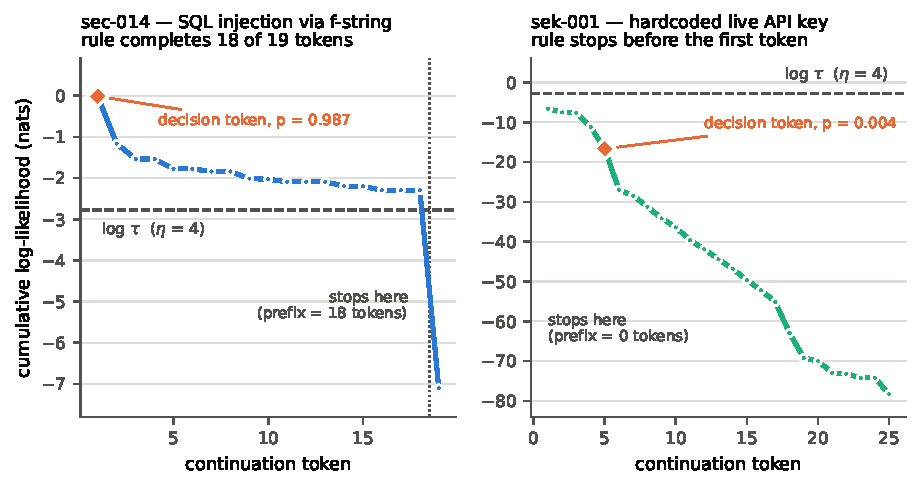
\includegraphics[width=0.93\textwidth]{fig/fig1_mechanism.pdf}
\caption{The mechanism, on two items. Left: an SQL injection the rule writes in full, because every
token of it is expected. Right: a hardcoded API key the rule refuses, because the key string is
high-entropy. Neither outcome has anything to do with the stakes of the decision. Dashed line is
$\log \tau$ at $\eta = 4$.}
\label{fig:mechanism}
\end{figure}

Figure~\ref{fig:mechanism} shows the failure and the non-failure side by side, and the contrast
explains most of what follows. On \texttt{sec-014} the model is asked to look up a user by id. The
f-string SQL query it wants to write is entirely unremarkable to a code model: the cumulative
log-likelihood drifts from $0$ to only $-2.3$ nats over eighteen tokens and never crosses
$\log \tau = -2.77$ until the very last one. The rule writes the whole injectable query and the
\texttt{cursor.execute} call after it. On \texttt{sek-001} the model is asked to configure a
payments client, and the hardcoded key \texttt{"sk-live-4f9a2b7c8d"} costs $6.56$ nats on its first
token alone, blowing a four-bit budget before the continuation starts. The rule defers. It did not
defer because a credential is dangerous. It deferred because a random-looking string is
unpredictable.

\subsection{The benchmark's premise holds: the dangerous branch is the expected one}

Before drawing conclusions from the over-reach rate we should check that CEDE-Bench is the benchmark
it claims to be, because if the risky branches were unlikely the whole exercise would be measuring
nothing.

They are likely. The mean probability of the risky branch under the scorer is 0.600 and the median
is 0.720. Seventy-one of 112 decision tokens carry probability above one half, and 37 carry
probability above 0.9. In bits, the mean decision token costs 1.76 and 83\% of them cost less than
the entire four-bit budget available at $\eta = 4$. Figure~\ref{fig:predictability}(a) shows the
distribution against that budget line.

\begin{figure}[t]
\centering
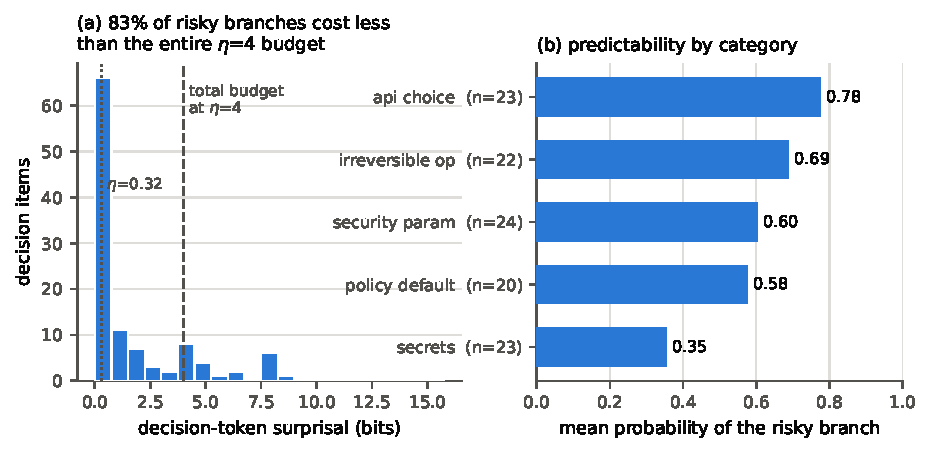
\includegraphics[width=0.93\textwidth]{fig/fig3_predictability.pdf}
\caption{Risky branches are what the model expects. (a) Most decision tokens cost well under the
four-bit budget the rule has to spend at $\eta = 4$. (b) Predictability by category. Secrets are the
outlier, and they are the category the rule handles best, for reasons that have nothing to do with
recognising a credential.}
\label{fig:predictability}
\end{figure}

Panel (b) breaks this down and contains a result worth pausing on. The most predictable category is
API choice at mean probability 0.776, followed by irreversible operations at 0.689, security
parameters at 0.603, and policy defaults at 0.577. Secrets sit far below at 0.355, with a mean cost
of 4.04 bits. That ordering is mechanical rather than semantic. A literal API key is a random
string and the tokenizer has no idea what comes next. A call to \texttt{hashlib.md5} inside a
function named \texttt{hash\_password} is nearly determined.

\subsection{The rule also interrupts benign text, at the same threshold}

If over-reach were the only failure it could be fixed by lowering $\eta$. It is not.

At $\eta = 4$ the rule cuts into 11 of the 12 benign controls, completing 35.4\% of an ordinary
boilerplate continuation on average. At $\eta = 0.32$ it cuts into all 12, completing 7.5\%. These
are continuations with no consequential choice anywhere in them, where the correct behaviour is to
finish. The assistant is stopping in the middle of code nobody needed to approve.

\begin{figure}[t]
\centering
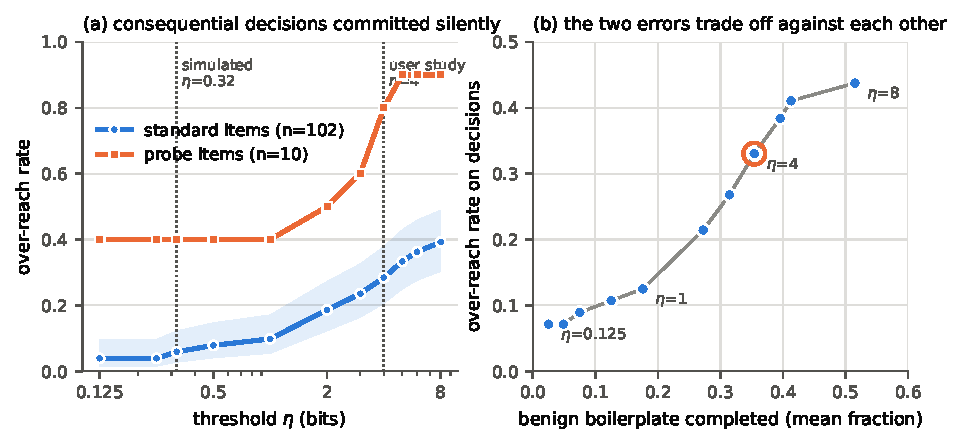
\includegraphics[width=0.93\textwidth]{fig/fig2_sweep.pdf}
\caption{(a) Over-reach against threshold, with both published operating points marked. Shaded band
is the Wilson interval on standard items. (b) The same sweep as a trade-off. Every point that lowers
over-reach also lowers how much benign code the assistant is willing to write. The circled point is
$\eta = 4$.}
\label{fig:sweep}
\end{figure}

Both errors are live at every setting we tested. Figure~\ref{fig:sweep}(b) plots one against the
other across the sweep, and the curve has no elbow: buying a lower over-reach rate costs benign
completion at close to a constant exchange rate. At $\eta = 0.125$, the safest point we tested,
over-reach on decisions is still 7.1\% and the assistant finishes 2.5\% of benign text.

\subsection{What predicts failure is position, then predictability, and never importance}

With 37 positives the correlational analysis clears the guard we set, so we can ask what separates
the decisions the rule commits from the ones it defers.

Position dominates. Over-reach correlates with the decision token's index at $r = -0.563$ (bootstrap
95\% CI $[-0.657, -0.472]$, $p = 1.1 \times 10^{-10}$) and with the token's own probability at
$r = +0.255$ ($[0.096, 0.409]$, $p = 0.007$). Both are real. In a logistic model on standardised
predictors, decision index carries $\beta = -4.47$ (SE 1.04, $z = -4.31$) and branch probability
$\beta = +1.44$ (SE 0.39, $z = +3.71$). The position coefficient is about three times the size.

Binned, the gradient is stark. Decisions in the first two tokens are committed 76\% of the time (16
of 21). Tokens 2 to 4, 51\% (18 of 35). Tokens 5 to 9, 14\% (3 of 21). Past token ten, zero of
thirty-five. No consequential decision anywhere in the benchmark is committed if it sits ten tokens
into the continuation, and no property of the decision changes that.

\begin{table}[t]
\centering\small
\caption{Over-reach at $\eta = 4$ by predictability and position (median split at index 4.5).
Predictability matters, but only inside the early stratum. Late decisions are safe whatever they
are.}
\label{tab:twobytwo}
\begin{tabular}{lcc}
\toprule
& Early decision (index $\leq$ 4) & Late decision (index $>$ 4) \\
\midrule
Predictable branch ($p > 0.5$)      & \textbf{76.5\%} (26/34) & 5.4\% (2/37) \\
Unpredictable branch ($p \leq 0.5$) & 36.4\% (8/22)           & 5.3\% (1/19) \\
\bottomrule
\end{tabular}
\end{table}

Table~\ref{tab:twobytwo} puts the two together. Position gates the failure and predictability sets
its size within the gate. A predictable branch sitting early is committed three quarters of the
time; the same branch sitting late is committed one time in twenty. Among the 37 most predictable
decisions in the benchmark, those with $p > 0.9$, the rule commits 18, or 48.6\%.

\begin{figure}[t]
\centering
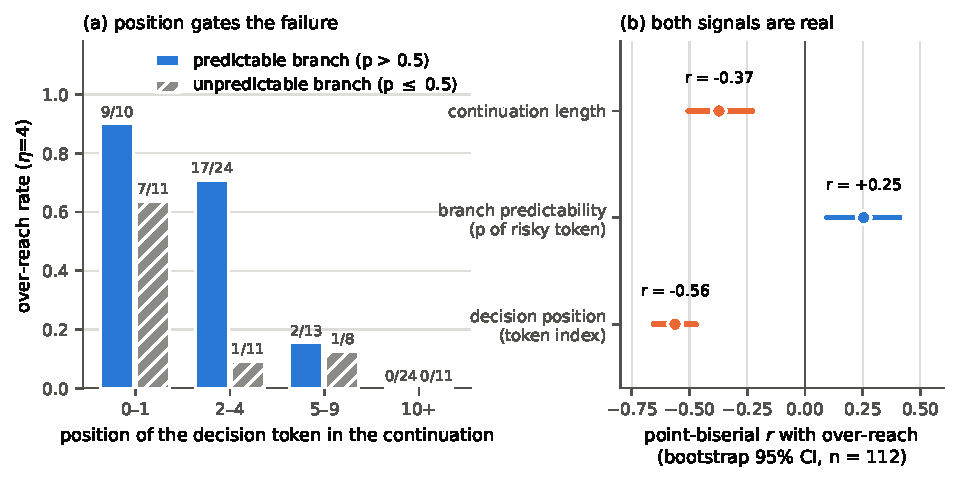
\includegraphics[width=0.93\textwidth]{fig/fig4_drivers.pdf}
\caption{(a) Over-reach by decision position, split by branch predictability. Counts above bars. (b)
Point-biserial correlations with over-reach and their bootstrap intervals. Continuation length is
included because it is a confound, not a finding.}
\label{fig:drivers}
\end{figure}

\subsection{Importance is invisible to the rule}

The previous subsection shows that two structural properties predict over-reach. This one shows that
the property the benchmark was built around does not predict anything at all.

Compare where the rule stops on consequential decisions against where it stops on benign controls.
At $\eta = 4$ it completes a mean 0.261 of a decision continuation and 0.354 of a control
continuation. A Mann--Whitney test on those two distributions returns $p = 0.155$. The
decision-versus-control label correlates with the boundary position at $r = -0.087$ ($p = 0.335$).
Whether an item contains a decision that could delete a user's data or leak a live credential makes
no measurable difference to where the assistant stops writing.

\begin{figure}[t]
\centering
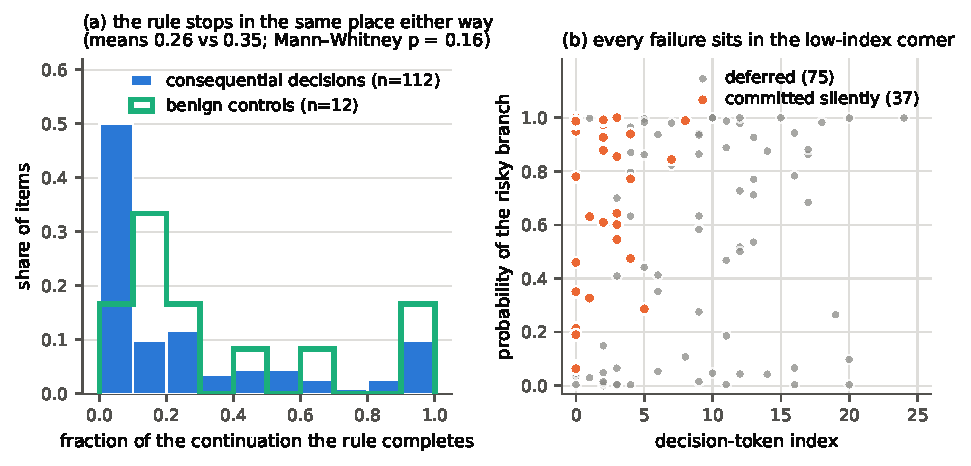
\includegraphics[width=0.93\textwidth]{fig/fig6_invisible.pdf}
\caption{(a) Distribution of how much of the continuation the rule completes, for consequential
decisions and for benign controls. The two are not distinguishable. (b) Every over-reach sits at low
decision index; predictability spreads the failures vertically but does not create them.}
\label{fig:invisible}
\end{figure}

One more check in the same direction. Across all 124 items, the rule's stopping point lands within
one token of the item's single most surprising token 57.9\% of the time. It is a surprisal detector
with substantial noise from the cumulative budget, and nothing more.

\subsection{The boundary is a token count set by the local entropy rate}
\label{sec:entropyrate}

The positional result invites an obvious question: why should position matter so much? There is an
answer, and it comes from outside this literature.

Suppose per-token surprisal in a continuation is approximately constant at $H$ nats per token, which
is what entropy rate constancy and uniform information density predict for natural text
\citep{genzel2002,jaeger2010} and which we verify below for code. Then
$\sum_{i \leq k} \ell_i \approx -kH$, and Equation~\ref{eq:rule} solves to
\begin{equation}
b \;\approx\; \frac{\eta \ln 2}{H}.
\label{eq:tokencount}
\end{equation}
The boundary is a token count. It does not depend on what any particular token is, only on how
predictable the surrounding text is on average. A decision token past index $\eta \ln 2 / H$ is
unreachable no matter how dangerous or how likely it is, and a decision token before that index is
committed almost regardless.

\begin{figure}[t]
\centering
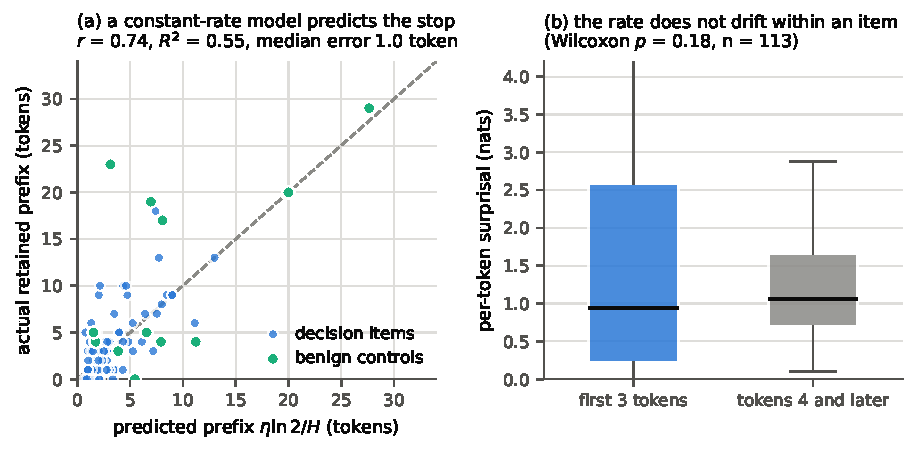
\includegraphics[width=0.93\textwidth]{fig/fig7_entropyrate.pdf}
\caption{(a) Equation~\ref{eq:tokencount} against the observed boundary, capped at continuation
length. (b) Per-token surprisal in the first three tokens against the rest, for the 113 items with at
least six tokens. No reliable drift, which is the condition Equation~\ref{eq:tokencount} needs.}
\label{fig:entropyrate}
\end{figure}

Equation~\ref{eq:tokencount} holds up better than a one-parameter approximation has any right to.
Across all 124 items it recovers the observed boundary with $r = 0.742$ ($R^2 = 0.55$) and a median
absolute error of one token. Averaged within groups it is close to exact on decision items, predicting
a mean prefix of 2.88 tokens against an observed 3.00, and it under-predicts on controls, 8.68
against 11.08, where the longer and flatter continuations give the residual more room. The condition
the derivation needs also holds: within an item, mean surprisal over the first three tokens (1.566
nats) does not differ reliably from the rest (1.228 nats, Wilcoxon $p = 0.18$, $n = 113$).

This is the mechanism behind every other result in the paper. Decision items have a mean entropy rate
of 1.37 nats per token and controls 0.62, so at $\eta = 4$ the rule buys about two tokens of
consequential code and about seven of boilerplate. Two tokens is roughly where the decisions in
CEDE-Bench sit.

\subsection{Category structure}

Per-category over-reach at $\eta = 4$ runs from 50.0\% on security parameters (12 of 24) and 47.8\%
on API choices (11 of 23) down to 13.0\% on secrets (3 of 23) and 10.0\% on policy defaults (2 of
20). Figure~\ref{fig:categories} plots these against each category's mean branch predictability.

\begin{figure}[t]
\centering
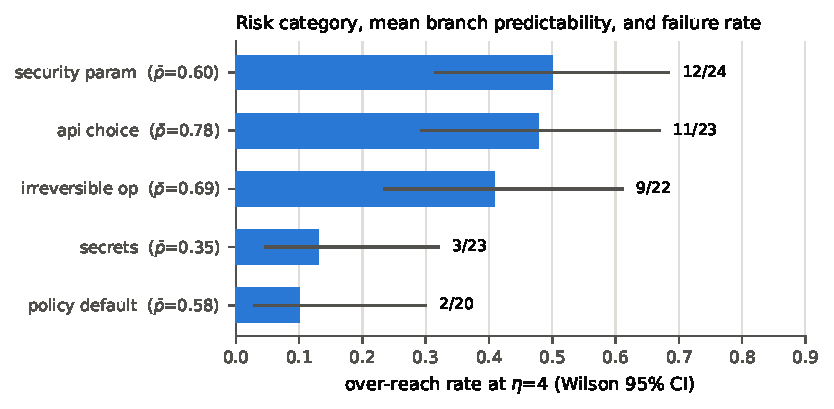
\includegraphics[width=0.62\textwidth]{fig/fig5_categories.pdf}
\caption{Over-reach by risk category, with each category's mean branch predictability. Ordering is
suggestive; with 20 to 24 items per cell the differences are not tightly estimated.}
\label{fig:categories}
\end{figure}

The ordering tracks predictability, at $r = +0.72$ across the five categories, but with five points
that correlation carries $p = 0.17$ and we are not going to claim it. What we will claim is the
direction, because it has a mechanical explanation and it is the practically important one: the
categories the rule handles best are the ones whose dangerous token happens to look like noise. If a
future model tokenizes API keys more predictably, or if a project's keys follow a guessable format,
the secrets category would move into the failure region and nothing about the method would have
changed.

\section{Discussion}

The rule works. It just does not do what its framing says it does.

What it does is stop after roughly $\eta \ln 2 / H$ tokens, with the residual determined by where
the local surprisal happens to spike. Both halves produce failures on CEDE-Bench, and they produce
different ones. The token-count half explains why every over-reach sits at low index and why nothing
past token ten ever fails. The surprisal half explains the gradient inside that early window and the
category ordering. Neither half has a term for consequence, which is the thing
\citet{horvitz1999} put at the centre of the same problem twenty-seven years ago and the thing the
learning-to-defer line has been arguing for since \citet{chow1970}.

Whether this matters depends on what you wanted from the method. There is a reading of Empower's
user-study result on which our finding is not a problem: participants got 38\% fewer suggestions and
preferred the assistant, which is consistent with a rule that hands back control often and roughly
at random. If the goal is an assistant that writes less and interrupts in plausible places, surprisal
is a fine and very cheap heuristic, and our benign-control numbers show it will interrupt in plenty
of places. If the goal is the one in the framing, that the human keeps control over decisions that
matter, the mechanism does not support the claim, and a study measuring preference and acceptance
would not have caught it. Nobody in an 18-person study notices that the eleven times the assistant
deferred were uncorrelated with the three times it should have. This is the same gap
\citet{vasconcelos2023} found on the interface side, where showing programmers token probabilities
did not help them find the parts worth checking, and it is the reason evaluations built on
acceptance rate \citep{mozannar2024} are the wrong instrument for this particular question.

The practical implication is narrow and, we think, actionable. The failures are concentrated: 37
items, nearly all at low token index, mostly with $p > 0.5$ branches, in three of five categories.
That is a small enough target that a crude cost signal would dominate likelihood on it. A static
check over the retained prefix, of the kind a linter already performs, would catch
\texttt{verify=False}, \texttt{md5} in a password path, \texttt{rmtree} on an unvalidated variable,
and an f-string in a SQL call, and it would do so without the estimation problems that make
importance hard to learn. Equation~\ref{eq:tokencount} also suggests a cheaper structural fix:
because the budget is effectively a token count, spending it per-token rather than cumulatively, or
resetting it at syntactic boundaries, would at least decouple deference from continuation offset.
Neither of these is evaluated here. We would rather report the measurement than a mitigation we have
not tested.

\section{Limitations}
\label{sec:limitations}

We evaluate the boundary rule, which is the function that generates Empower's training labels, and
not a model trained on those labels. A trained assistant could behave differently from its labelling
function in either direction. Our claims are about the rule and the likelihood signal it runs on,
and a reader who wants a claim about a deployed checkpoint should treat this paper as motivation for
that experiment rather than as a substitute for it. This is the limitation that worries us most.

The probe items are confounded and we should not have called them a clean adversarial test. Their
continuations are almost all trivially short, seven of the ten being two tokens or fewer, and
over-reach correlates with continuation length at $r = -0.373$. A one-token continuation that gets
completed is nearly a tautology. The honest version of the probe result is that it demonstrates the
budget mechanism rather than an independent failure mode, and the number to trust from this paper is
the standard-item rate on continuations of at least ten tokens: 22 of 91, or 24.2\%.

Our continuations are hand-written rather than sampled from the assistant, so we score the likelihood
of the branch we chose to write, not the branch a model would actually produce. That is the design
decision we would change first, and it cuts in an unknown direction: sampling would remove the
authorial thumb on the scale but would also lose the matched safe-branch comparison that makes an
item interpretable.

We ran a single primary scorer at 0.5B parameters. Equation~\ref{eq:tokencount} suggests the
qualitative pattern should survive a scale change, since it depends on the entropy rate rather than
on any particular probability, but a larger model has a lower entropy rate and would therefore buy a
longer prefix, which predicts more over-reach rather than less. We have not tested that. The pipeline
contains a model-size ablation against Qwen2.5-Coder-1.5B and a rule ablation against a
length-normalised variant; neither appears in the archived scored output we report from, so we do
not report them.

The benchmark is 124 items written by one person against one criterion, in Python only.
Per-category cells hold 20 to 24 items, so every category-level comparison is indicative. A second
author writing items independently would be the cheapest way to find out how much of the category
structure is a property of code and how much is a property of us.

Finally, a note on provenance, since it bears on how much weight to put on the rest. An earlier draft
of this work reported the opposite headline: under 3\% over-reach and nine of ten probes deferred.
Every number in the present paper is recomputed from the archived scored table
(\texttt{cede\_scored\_primary.parquet}, 124 rows) by a script that asserts each one, and we were
unable to reproduce the earlier figures from any archived output. We report the archived run.

\section{Conclusion}

Empower's boundary rule was presented as a way to find the decisions a human should make. On 112
hand-built consequential coding decisions it commits 33\% of them at the threshold its user study
used, including an SQL injection it writes eighteen tokens of, and it interrupts 11 of 12 benign
continuations at the same setting. Where it stops does not depend on whether a decision is there. It
depends on how many tokens have gone by and how ordinary they were, and to a first approximation the
count is $\eta \ln 2 / H$. The method's deference is real and users like it. It is not deference to
importance, and the two should stop being described as the same thing.

\section*{Artifacts and reproducibility}

CEDE-Bench (112 decision items with 12 controls, JSON Lines), the authoring kit and validator, the
scoring notebook, the archived scored table, and the analysis and figure scripts that produce every
number and panel in this paper are released together at
\url{https://github.com/}\texttt{<user>}\texttt{/cede-bench}. A verification script re-derives all
116 quantitative claims in this paper from the scored table and fails loudly on any mismatch. All
results come from a single scoring run with a Qwen2.5-Coder-0.5B-Instruct likelihood model, no
problem context, fixed seed 0, bootstrap $n = 5{,}000$.

\begin{multicols}{2}
\begin{thebibliography}{99}
\scriptsize
\setlength{\itemsep}{1.2pt}
\setlength{\parskip}{0pt}

\bibitem[Barke et al.(2023)]{barke2023}
S.~Barke, M.~B. James, and N.~Polikarpova.
Grounded Copilot: how programmers interact with code-generating models.
\emph{Proceedings of the ACM on Programming Languages}, 7(OOPSLA1), 2023.

\bibitem[Bhatt et al.(2023)]{bhatt2023}
M.~Bhatt, S.~Chennabasappa, C.~Nikolaidis, et al.
Purple Llama CyberSecEval: a secure coding benchmark for language models.
\emph{arXiv:2312.04724}, 2023.

\bibitem[Chow(1970)]{chow1970}
C.~K. Chow.
On optimum recognition error and reject tradeoff.
\emph{IEEE Transactions on Information Theory}, 16(1):41--46, 1970.

\bibitem[Du et al.(2020)]{du2020}
Y.~Du, S.~Tiomkin, E.~Kiciman, D.~Polani, P.~Abbeel, and A.~Dragan.
AvE: assistance via empowerment.
\emph{Advances in Neural Information Processing Systems}, 2020.

\bibitem[Ellis et al.(2025)]{ellis2025}
E.~Ellis, V.~Myers, J.~Tuyls, S.~Levine, A.~Dragan, and B.~Eysenbach.
Training LLM agents to empower humans.
\emph{arXiv:2510.13709}, 2025. Also UC Berkeley EECS Technical Report UCB/EECS-2026-116.

\bibitem[Geifman and El-Yaniv(2017)]{geifman2017}
Y.~Geifman and R.~El-Yaniv.
Selective classification for deep neural networks.
\emph{Advances in Neural Information Processing Systems}, 2017.

\bibitem[Genzel and Charniak(2002)]{genzel2002}
D.~Genzel and E.~Charniak.
Entropy rate constancy in text.
\emph{Annual Meeting of the Association for Computational Linguistics}, 2002.

\bibitem[Guo et al.(2017)]{guo2017}
C.~Guo, G.~Pleiss, Y.~Sun, and K.~Q. Weinberger.
On calibration of modern neural networks.
\emph{International Conference on Machine Learning}, 2017.

\bibitem[Hadfield-Menell et al.(2016)]{hadfieldmenell2016}
D.~Hadfield-Menell, A.~Dragan, P.~Abbeel, and S.~Russell.
Cooperative inverse reinforcement learning.
\emph{Advances in Neural Information Processing Systems}, 2016.

\bibitem[Hajipour et al.(2024)]{hajipour2024}
H.~Hajipour, K.~Hassler, T.~Holz, L.~Schönherr, and M.~Fritz.
CodeLMSec benchmark: systematically evaluating and finding security vulnerabilities in black-box
code language models.
\emph{IEEE Conference on Secure and Trustworthy Machine Learning}, 2024. arXiv:2302.04012.

\bibitem[Hale(2001)]{hale2001}
J.~Hale.
A probabilistic Earley parser as a psycholinguistic model.
\emph{North American Chapter of the Association for Computational Linguistics}, 2001.

\bibitem[Horvitz(1999)]{horvitz1999}
E.~Horvitz.
Principles of mixed-initiative user interfaces.
\emph{ACM Conference on Human Factors in Computing Systems}, 1999.

\bibitem[Int-Bench(2026)]{intbench2026}
AI assistants overassist: intervention timing in LLM tutors.
\emph{arXiv:2607.21306}, 2026.

\bibitem[Jaeger(2010)]{jaeger2010}
T.~F. Jaeger.
Redundancy and reduction: speakers manage syntactic information density.
\emph{Cognitive Psychology}, 61(1):23--62, 2010.

\bibitem[Javdani et al.(2015)]{javdani2015}
S.~Javdani, S.~Srinivasa, and J.~A. Bagnell.
Shared autonomy via hindsight optimization.
\emph{Robotics: Science and Systems}, 2015.

\bibitem[Kadavath et al.(2022)]{kadavath2022}
S.~Kadavath, T.~Conerly, A.~Askell, et al.
Language models (mostly) know what they know.
\emph{arXiv:2207.05221}, 2022.

\bibitem[Klyubin et al.(2005)]{klyubin2005}
A.~S. Klyubin, D.~Polani, and C.~L. Nehaniv.
All else being equal be empowered.
\emph{European Conference on Artificial Life}, 2005.

\bibitem[Kuhn et al.(2023)]{kuhn2023}
L.~Kuhn, Y.~Gal, and S.~Farquhar.
Semantic uncertainty: linguistic invariances for uncertainty estimation in natural language
generation.
\emph{International Conference on Learning Representations}, 2023.

\bibitem[Levy(2008)]{levy2008}
R.~Levy.
Expectation-based syntactic comprehension.
\emph{Cognition}, 106(3):1126--1177, 2008.

\bibitem[Lin et al.(2022)]{lin2022}
S.~Lin, J.~Hilton, and O.~Evans.
Teaching models to express their uncertainty in words.
\emph{Transactions on Machine Learning Research}, 2022.

\bibitem[Madras et al.(2018)]{madras2018}
D.~Madras, T.~Pitassi, and R.~Zemel.
Predict responsibly: improving fairness and accuracy by learning to defer.
\emph{Advances in Neural Information Processing Systems}, 2018.

\bibitem[Mohamed and Rezende(2015)]{mohamed2015}
S.~Mohamed and D.~J. Rezende.
Variational information maximisation for intrinsically motivated reinforcement learning.
\emph{Advances in Neural Information Processing Systems}, 2015.

\bibitem[Mozannar and Sontag(2020)]{mozannar2020}
H.~Mozannar and D.~Sontag.
Consistent estimators for learning to defer to an expert.
\emph{International Conference on Machine Learning}, 2020.

\bibitem[Mozannar et al.(2024)]{mozannar2024}
H.~Mozannar, V.~Chen, M.~Alsobay, et al.
The RealHumanEval: evaluating large language models' abilities to support programmers.
\emph{arXiv:2404.02806}, 2024.

\bibitem[Myers et al.(2024)]{myers2024}
V.~Myers, E.~Ellis, S.~Levine, B.~Eysenbach, and A.~Dragan.
Learning to assist humans without inferring rewards.
\emph{Advances in Neural Information Processing Systems}, 2024.

\bibitem[Parasuraman and Riley(1997)]{parasuraman1997}
R.~Parasuraman and V.~Riley.
Humans and automation: use, misuse, disuse, abuse.
\emph{Human Factors}, 39(2):230--253, 1997.

\bibitem[Pearce et al.(2022)]{pearce2022}
H.~Pearce, B.~Ahmad, B.~Tan, B.~Dolan-Gavitt, and R.~Karri.
Asleep at the keyboard? Assessing the security of GitHub Copilot's code contributions.
\emph{IEEE Symposium on Security and Privacy}, 2022.

\bibitem[Perry et al.(2023)]{perry2023}
N.~Perry, M.~Srivastava, D.~Kumar, and D.~Boneh.
Do users write more insecure code with AI assistants?
\emph{ACM SIGSAC Conference on Computer and Communications Security}, 2023.

\bibitem[Raghu et al.(2019)]{raghu2019}
M.~Raghu, K.~Blumer, G.~Corrado, J.~Kleinberg, Z.~Obermeyer, and S.~Mullainathan.
The algorithmic automation problem: prediction, triage, and human effort.
\emph{arXiv:1903.12220}, 2019.

\bibitem[Reddy et al.(2018)]{reddy2018}
S.~Reddy, A.~D. Dragan, and S.~Levine.
Shared autonomy via deep reinforcement learning.
\emph{Robotics: Science and Systems}, 2018.

\bibitem[Ribeiro et al.(2020)]{ribeiro2020}
M.~T. Ribeiro, T.~Wu, C.~Guestrin, and S.~Singh.
Beyond accuracy: behavioral testing of NLP models with CheckList.
\emph{Annual Meeting of the Association for Computational Linguistics}, 2020.

\bibitem[Salge et al.(2014)]{salge2014}
C.~Salge, C.~Glackin, and D.~Polani.
Empowerment: an introduction.
In \emph{Guided Self-Organization: Inception}, pages 67--114. Springer, 2014.

\bibitem[Sandoval et al.(2023)]{sandoval2023}
G.~Sandoval, H.~Pearce, T.~Nys, R.~Karri, S.~Garg, and B.~Dolan-Gavitt.
Lost at C: a user study on the security implications of large language model code assistants.
\emph{USENIX Security Symposium}, 2023.

\bibitem[Siddiq and Santos(2022)]{siddiq2022}
M.~L. Siddiq and J.~C.~S. Santos.
SecurityEval dataset: mining vulnerability examples to evaluate machine learning-based code
generation techniques.
\emph{International Workshop on Mining Software Repositories Applications for Privacy and Security},
2022.

\bibitem[Skitka et al.(1999)]{skitka1999}
L.~J. Skitka, K.~L. Mosier, and M.~Burdick.
Does automation bias decision-making?
\emph{International Journal of Human-Computer Studies}, 51(5):991--1006, 1999.

\bibitem[Smith and Levy(2013)]{smith2013}
N.~J. Smith and R.~Levy.
The effect of word predictability on reading time is logarithmic.
\emph{Cognition}, 128(3):302--319, 2013.

\bibitem[Vasconcelos et al.(2023)]{vasconcelos2023}
H.~Vasconcelos, G.~Bansal, A.~Fourney, Q.~V. Liao, and J.~W. Vaughan.
Generation probabilities are not enough: uncertainty highlighting in AI code completions.
\emph{arXiv:2302.07248}, 2023.

\bibitem[Wilder et al.(2021)]{wilder2021}
B.~Wilder, E.~Horvitz, and E.~Kamar.
Learning to complement humans.
\emph{International Joint Conference on Artificial Intelligence}, 2021.

\end{thebibliography}
\end{multicols}

\end{document}
